\section{Appendix}
\label{sec:appendix}

\subsection{Regression Summary and Figures}
\begin{table}[ht]
    \centering
    \begin{tabular}{lcccc}
        \toprule
        \textbf{Coefficient} & \textbf{\ref{eq:univariate_linear_regression}} & \textbf{\ref{eq:dummy_univariate_linear_regression}} & \textbf{\ref{eq:multivariate_linear_regression}} & \textbf{\ref{eq:dummy_multivariate_linear_regression}} \\
        \midrule
        \text{Intercept} & 12.52 & 12.22 &  14.57 & 14.57 \\
                           & (0.00208) & (0.00202) & (1.826) & (1.826) \\
        \text{min\_dist} & -0.0000441 & & -0.000126 &  \\
                           & (0.000000470) &  & (0.00000145) &  \\
        \text{close}      &  & 0.314 &  & 0.189 \\
                           &  & (0.00283) &  & (0.00290) \\
        \text{min\_dist$^2$} & & & 1.09e-08 & \\
                              &  & & (1.35e-10) &  \\
        \midrule
        \textbf{Controls} & No & No & Yes & Yes \\
        \bottomrule
    \end{tabular}
    \label{tab:summary_regression_table}
    \caption{Regression Coefficients and Standard Errors for Model Specifications 1-4. Controls hold district, year, house age, and year-district interactions.}
\end{table}

% Figure showing log_price scatter (../figs/log_price_distance_scatter.png). Label: log_price_scatter
\begin{figure}
    \centering
    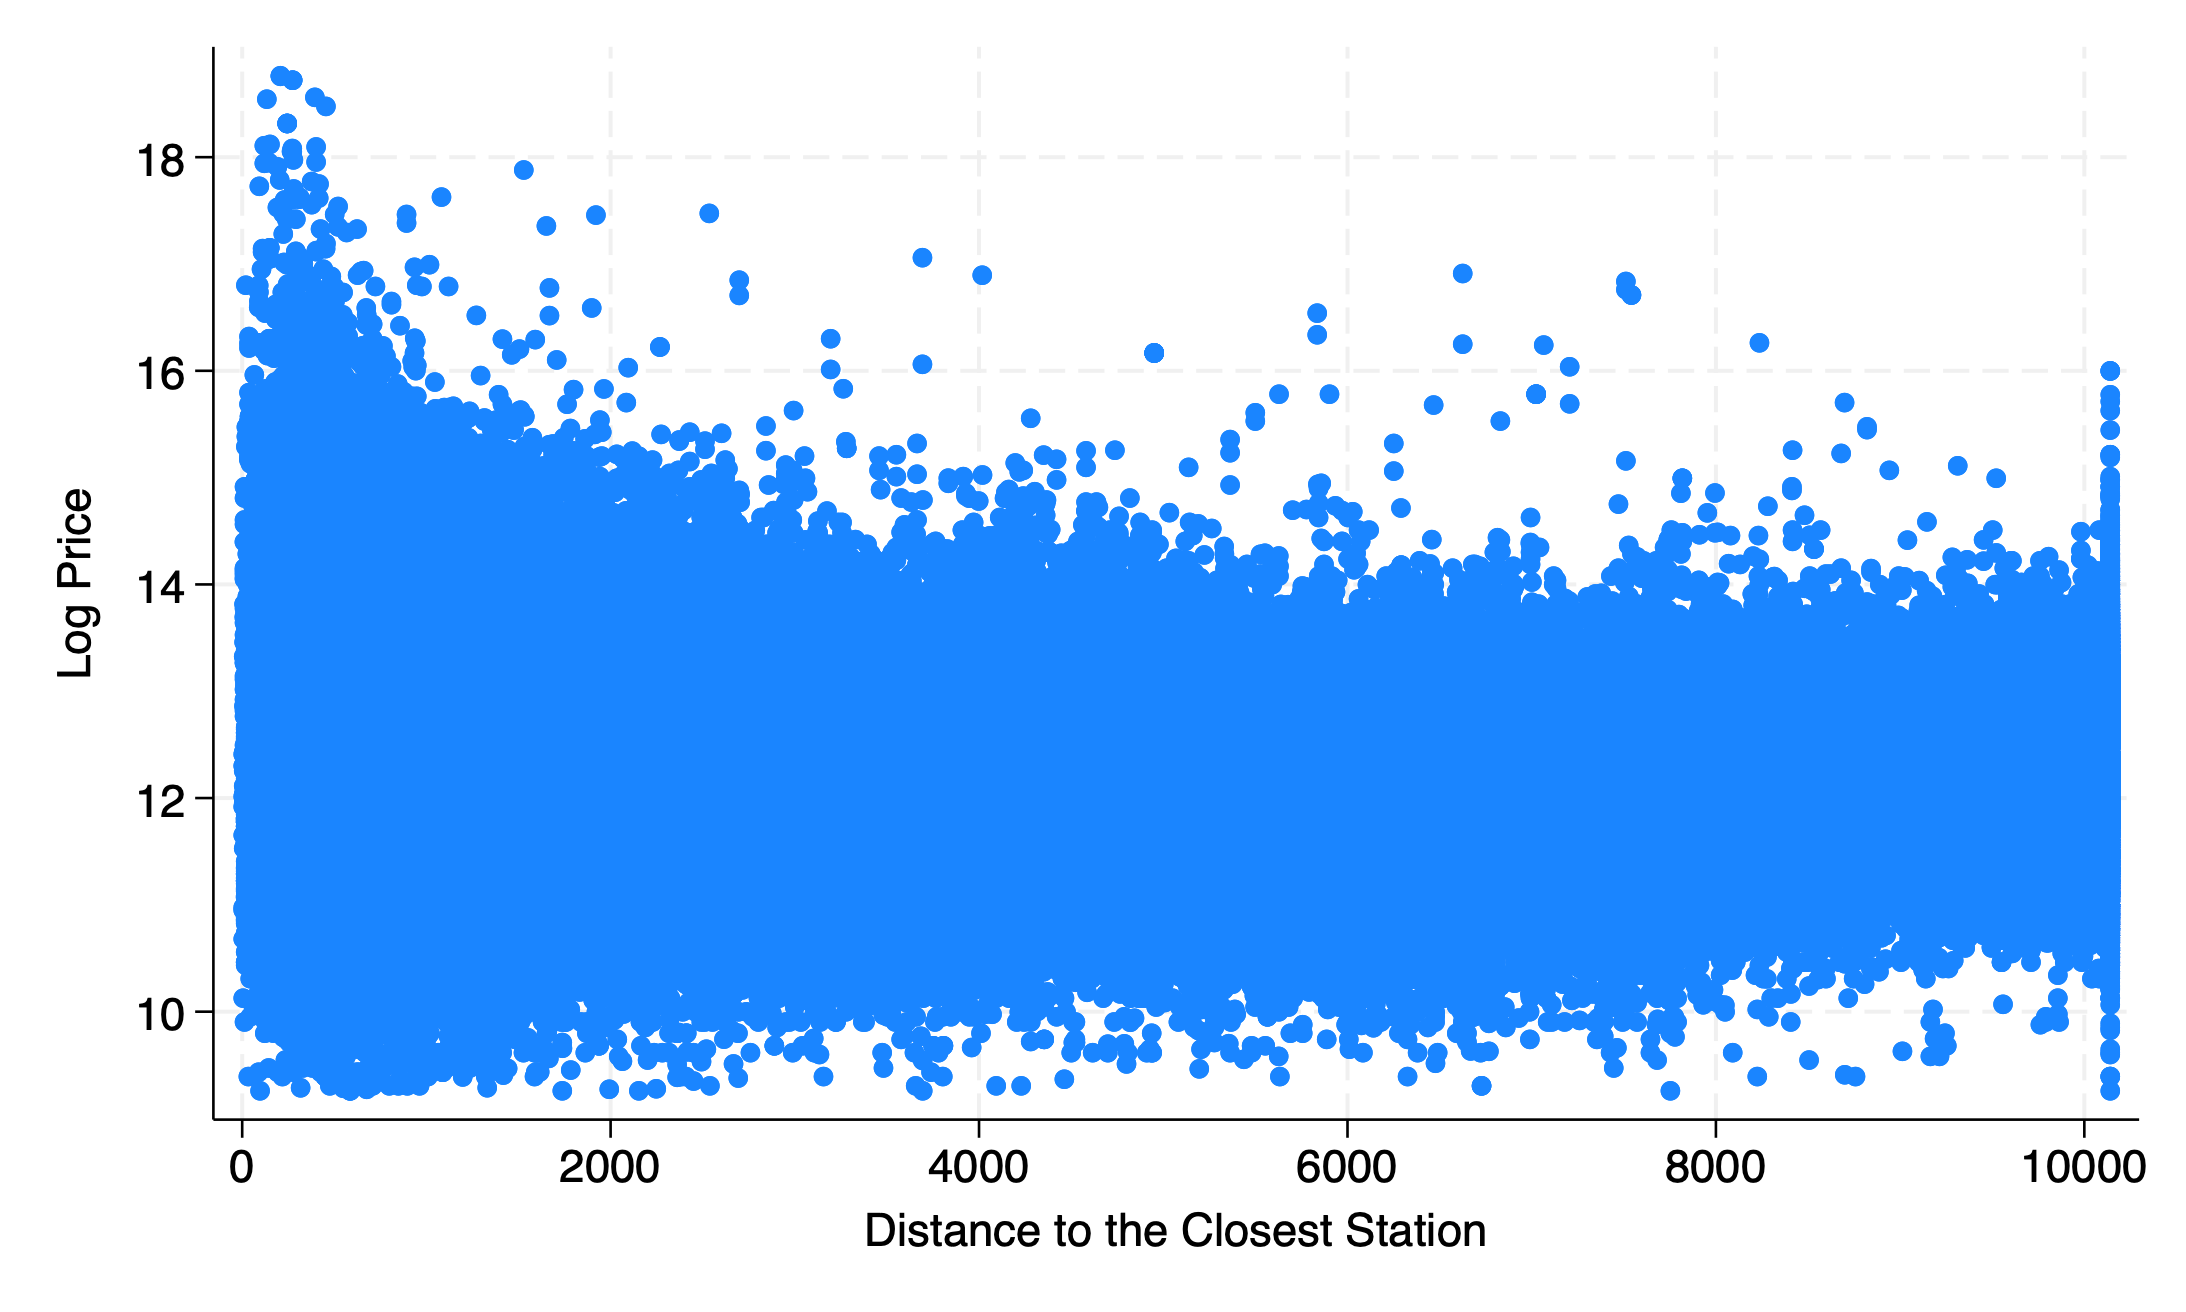
\includegraphics[width=0.8\textwidth]{../figs/log_price_distance_scatter.png}
    \caption{Scatter plot of log price against distance to the nearest subway station. Notice the non-linear relationship, and piece wise nature beyond 2km.}
    \label{log_price_scatter}
\end{figure}

% Figure shoiwng the distribution of min_dist (../figs/hist_min_dist.png). Label: min_dist_distribution
\begin{figure}
    \centering
    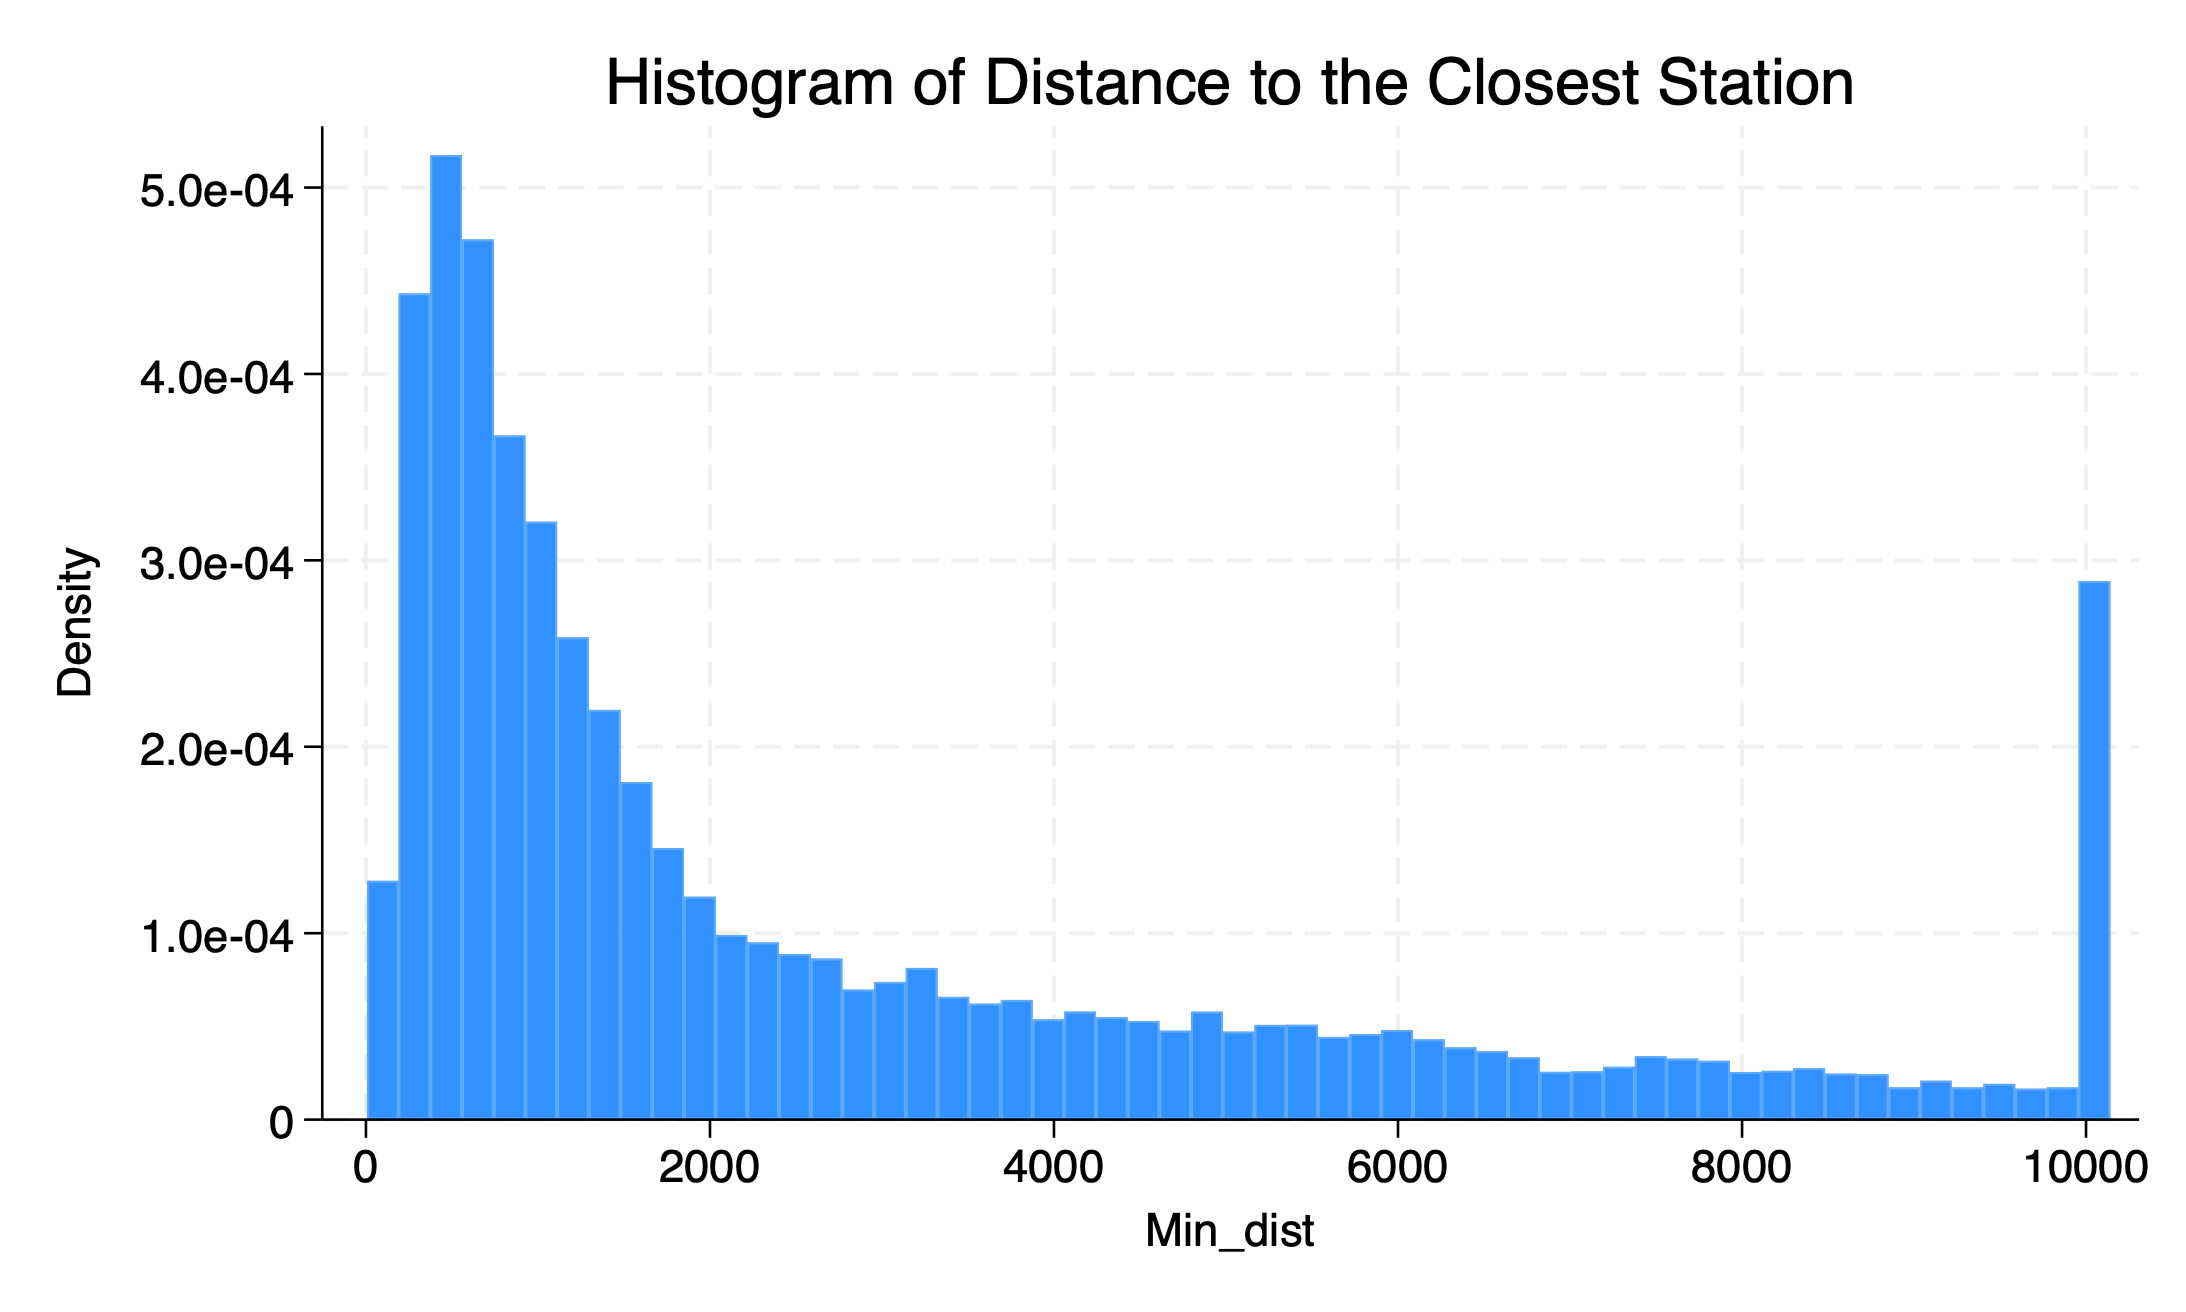
\includegraphics[width=0.8\textwidth]{../figs/hist_min_dist.png}
    \caption{Distribution of the minimum distance to a subway station. The raw distribution is right skewed with a long tail so we windsorize at 10km.}
    \label{min_dist_distribution}
\end{figure}

% Figure showing the distribution of log_price (../figs/hist_log_price.png). Label: log_price_distribution
\begin{figure}
    \centering
    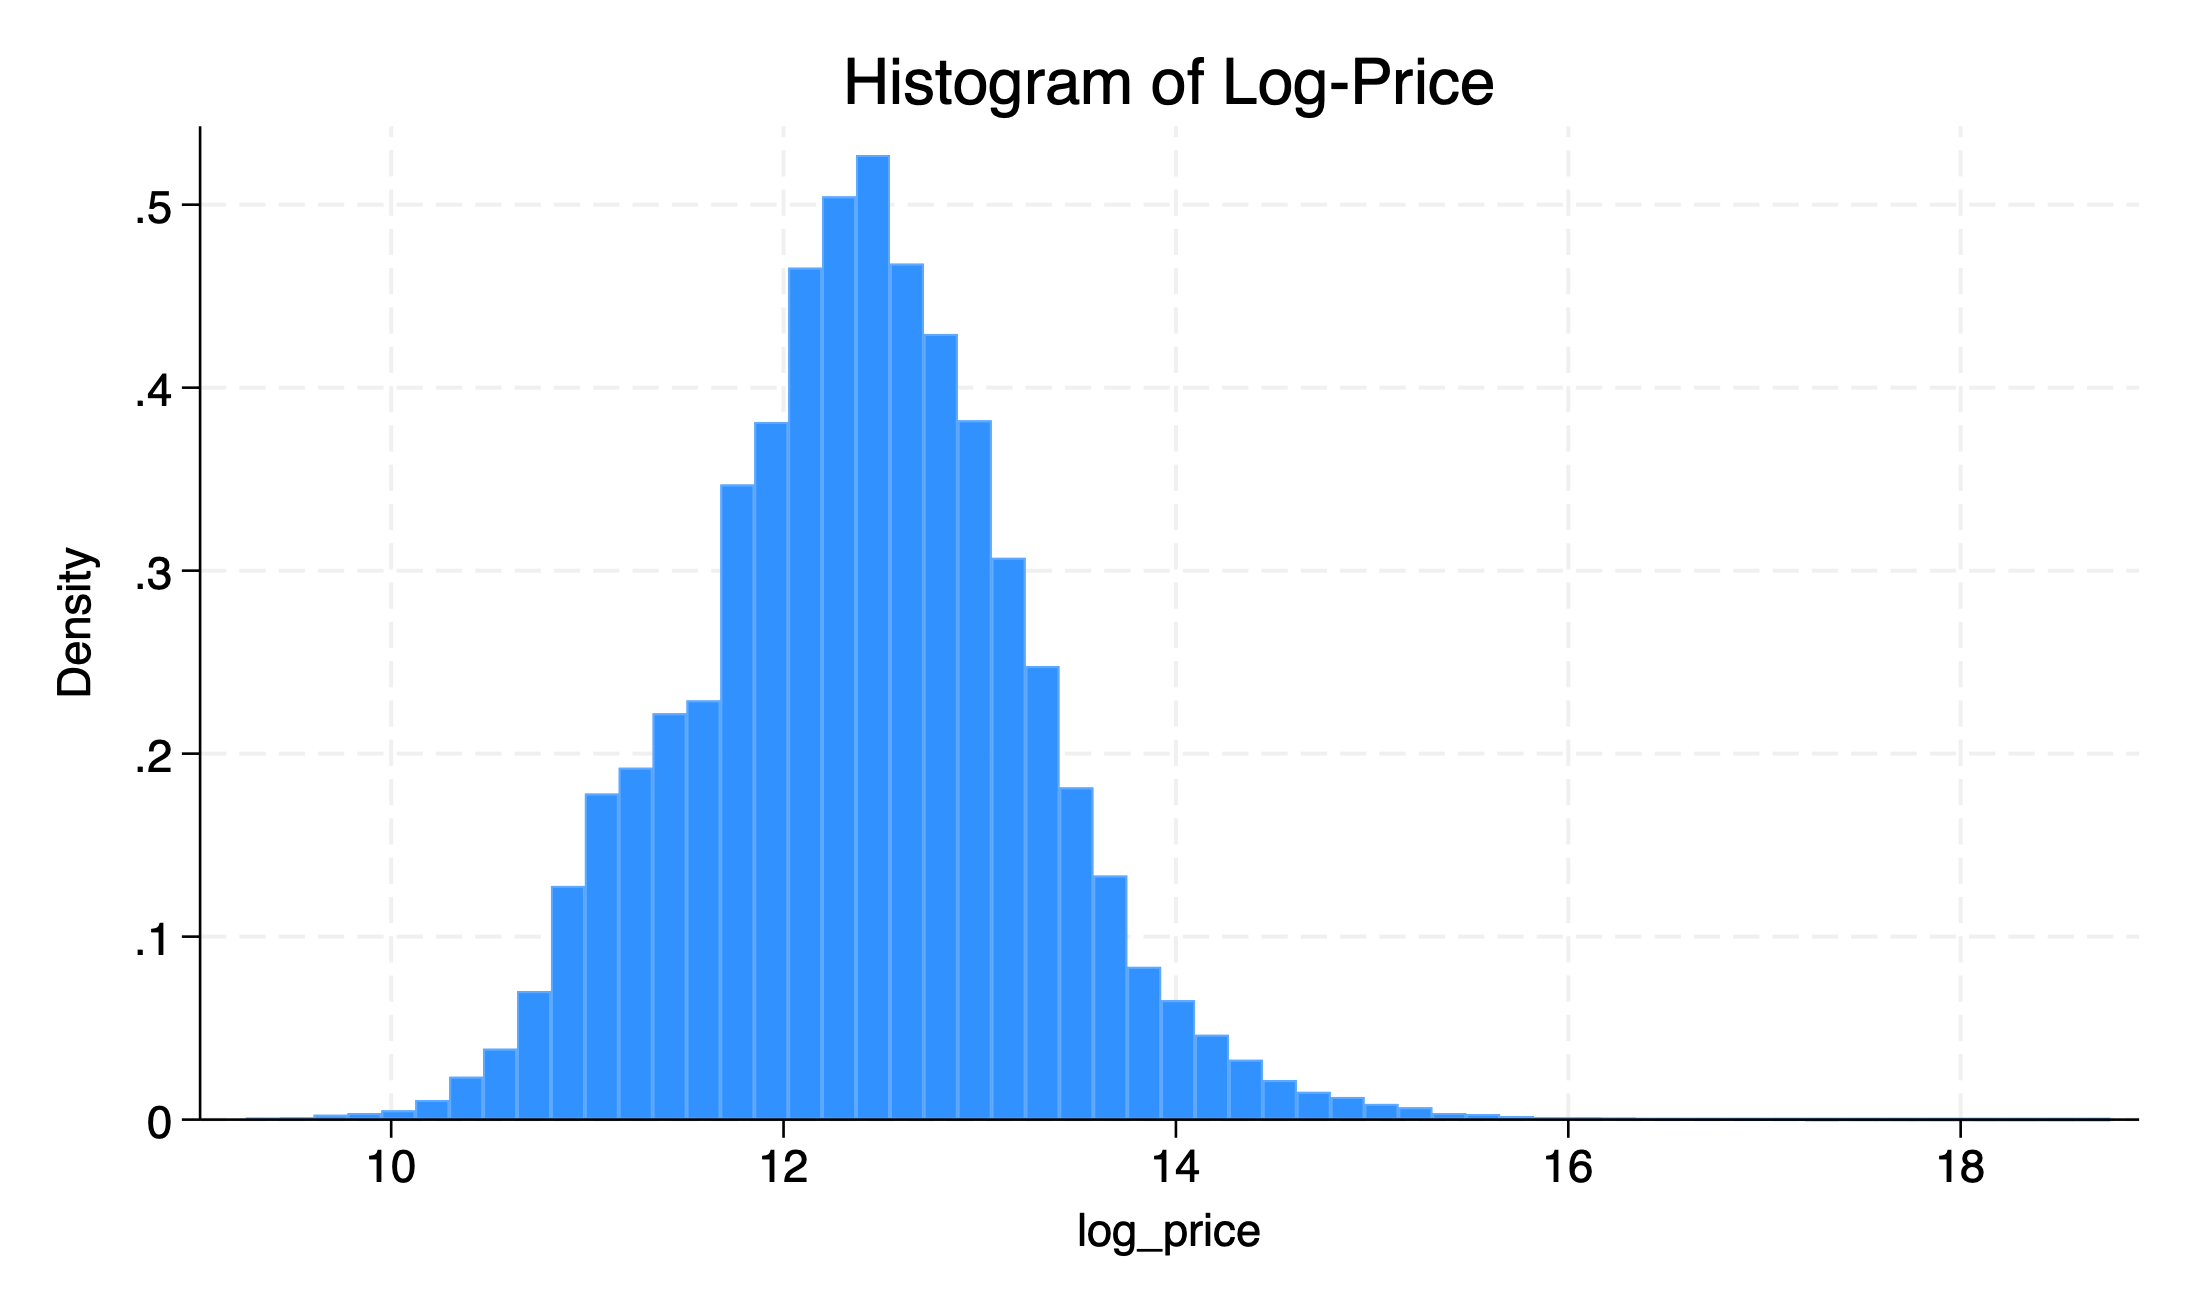
\includegraphics[width=0.8\textwidth]{../figs/hist_log_price.png}
    \caption{Distribution of log price. The log transformation accounts for the long tails in house price's distribution, and makes our regression nicely interpretable.}
    \label{log_price_distribution}
\end{figure}

% Figure showing fitted vs residuals for multivariate regression (../figs/MV_predicted_vs_actual.png). Label: MV_predicted_vs_actual
\begin{figure}
    \centering
    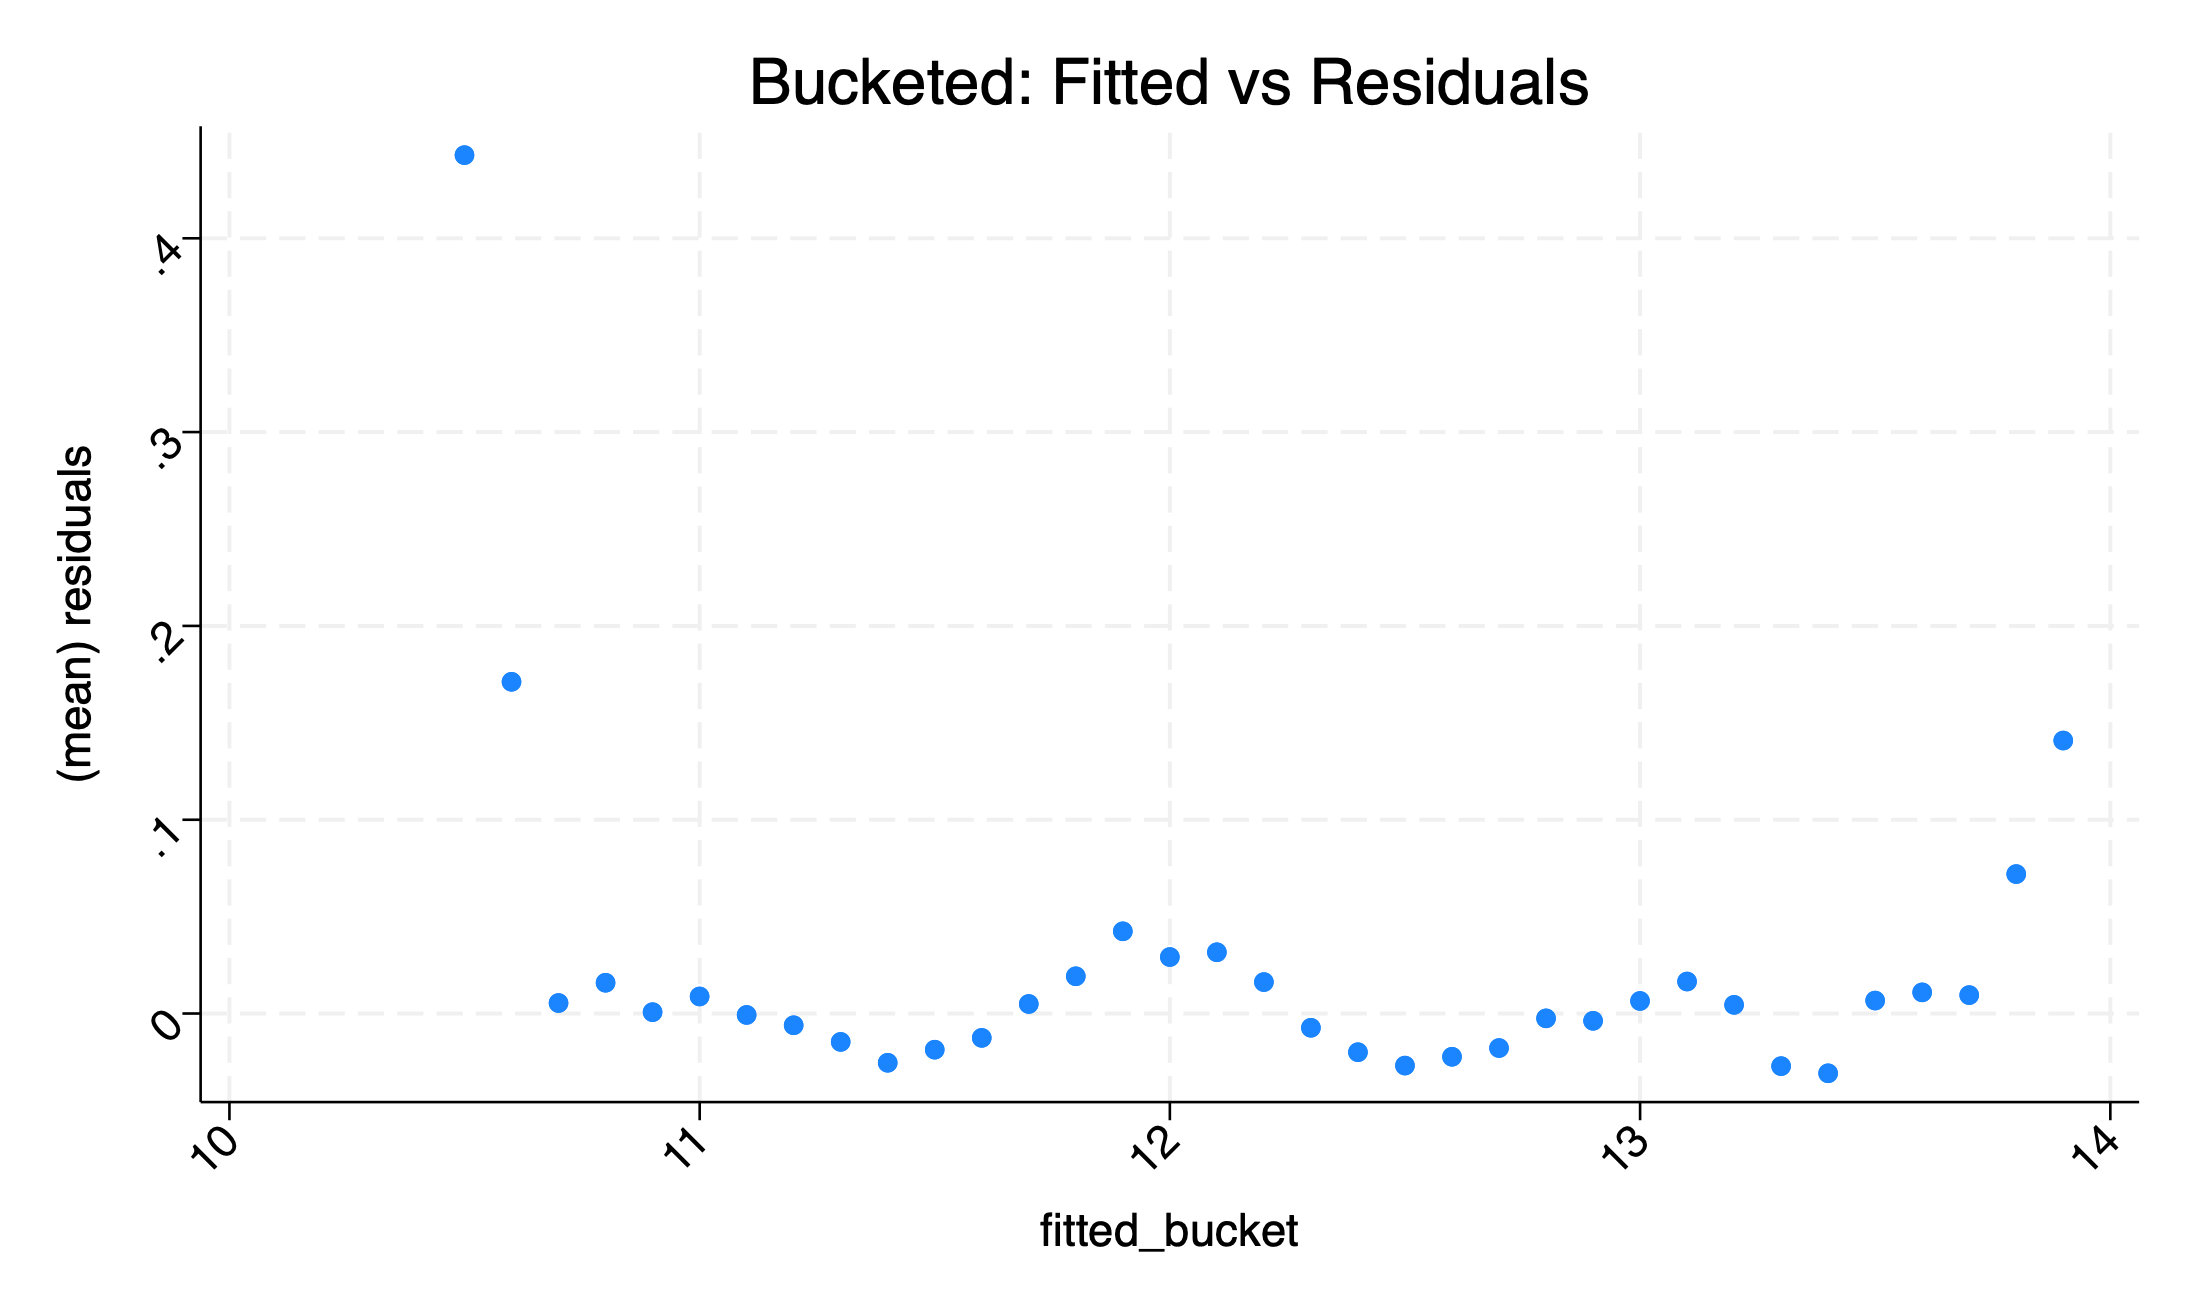
\includegraphics[width=0.8\textwidth]{../figs/MV_fitted_vs_residuals.png}
    \caption{Fitted vs Residuals plot for the multivariate regression. The residuals are distributed randomly around 0 apart from at the lower tail where they break down.
    Results are after bucketing predicteds into bins for easier interpretation.
    Results are from the regression in Specification \ref{eq:multivariate_linear_regression}.}
    \label{MV_fitted_vs_residuals}
\end{figure}

% Figure showing expected vs actual for multivariate regression (../figs/MV_bucketed_predicted_vs_actual.png). Label: MV_bucketed_predicted_vs_actual
\begin{figure}
    \centering
    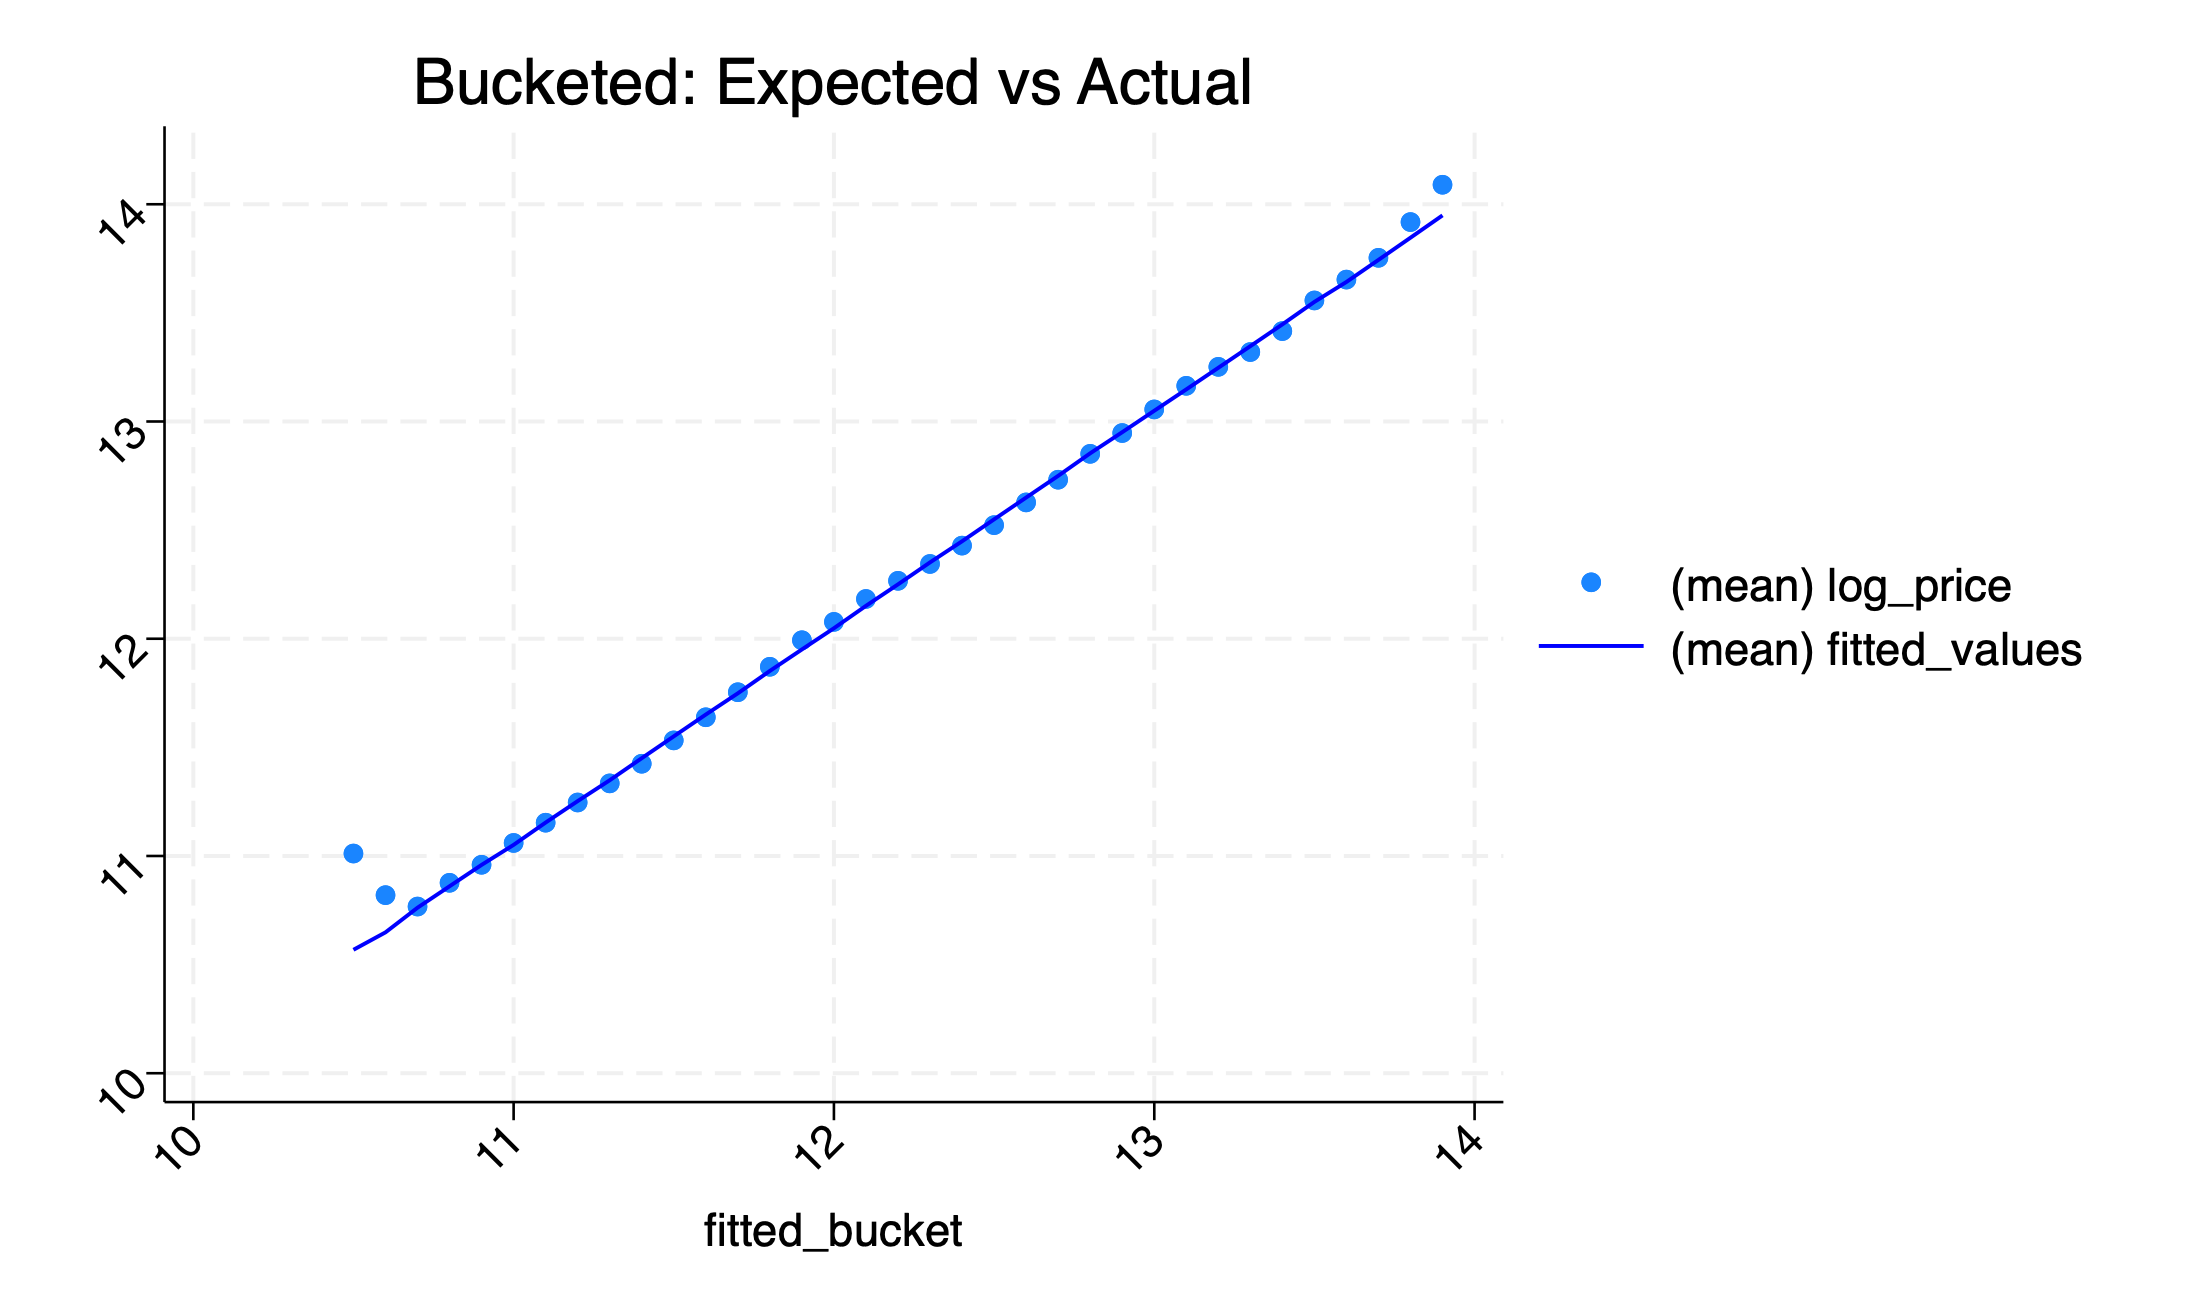
\includegraphics[width=0.8\textwidth]{../figs/MV_bucketed_expected_vs_actual.png}
    \caption{Bucketed Expected vs Actual plot for the multivariate regression. The expected values are bucketed into 10 bins and the actual values are averaged within each bin
    we do this becuase with over 340000 observations the plots otherwise are difficult to interpret. 
    Results are from the regression in Specification \ref{eq:multivariate_linear_regression}.}
    \label{MV_bucketed_predicted_vs_actual}
\end{figure}

% Same two but incl dummy
% Figure showing fitted vs residuals for multivariate regression with dummy (../figs/bucketed_dummy_expected_vs_actual.png). Label: MV_dummy_bucketed_predicted_vs_actual
\begin{figure}
    \centering
    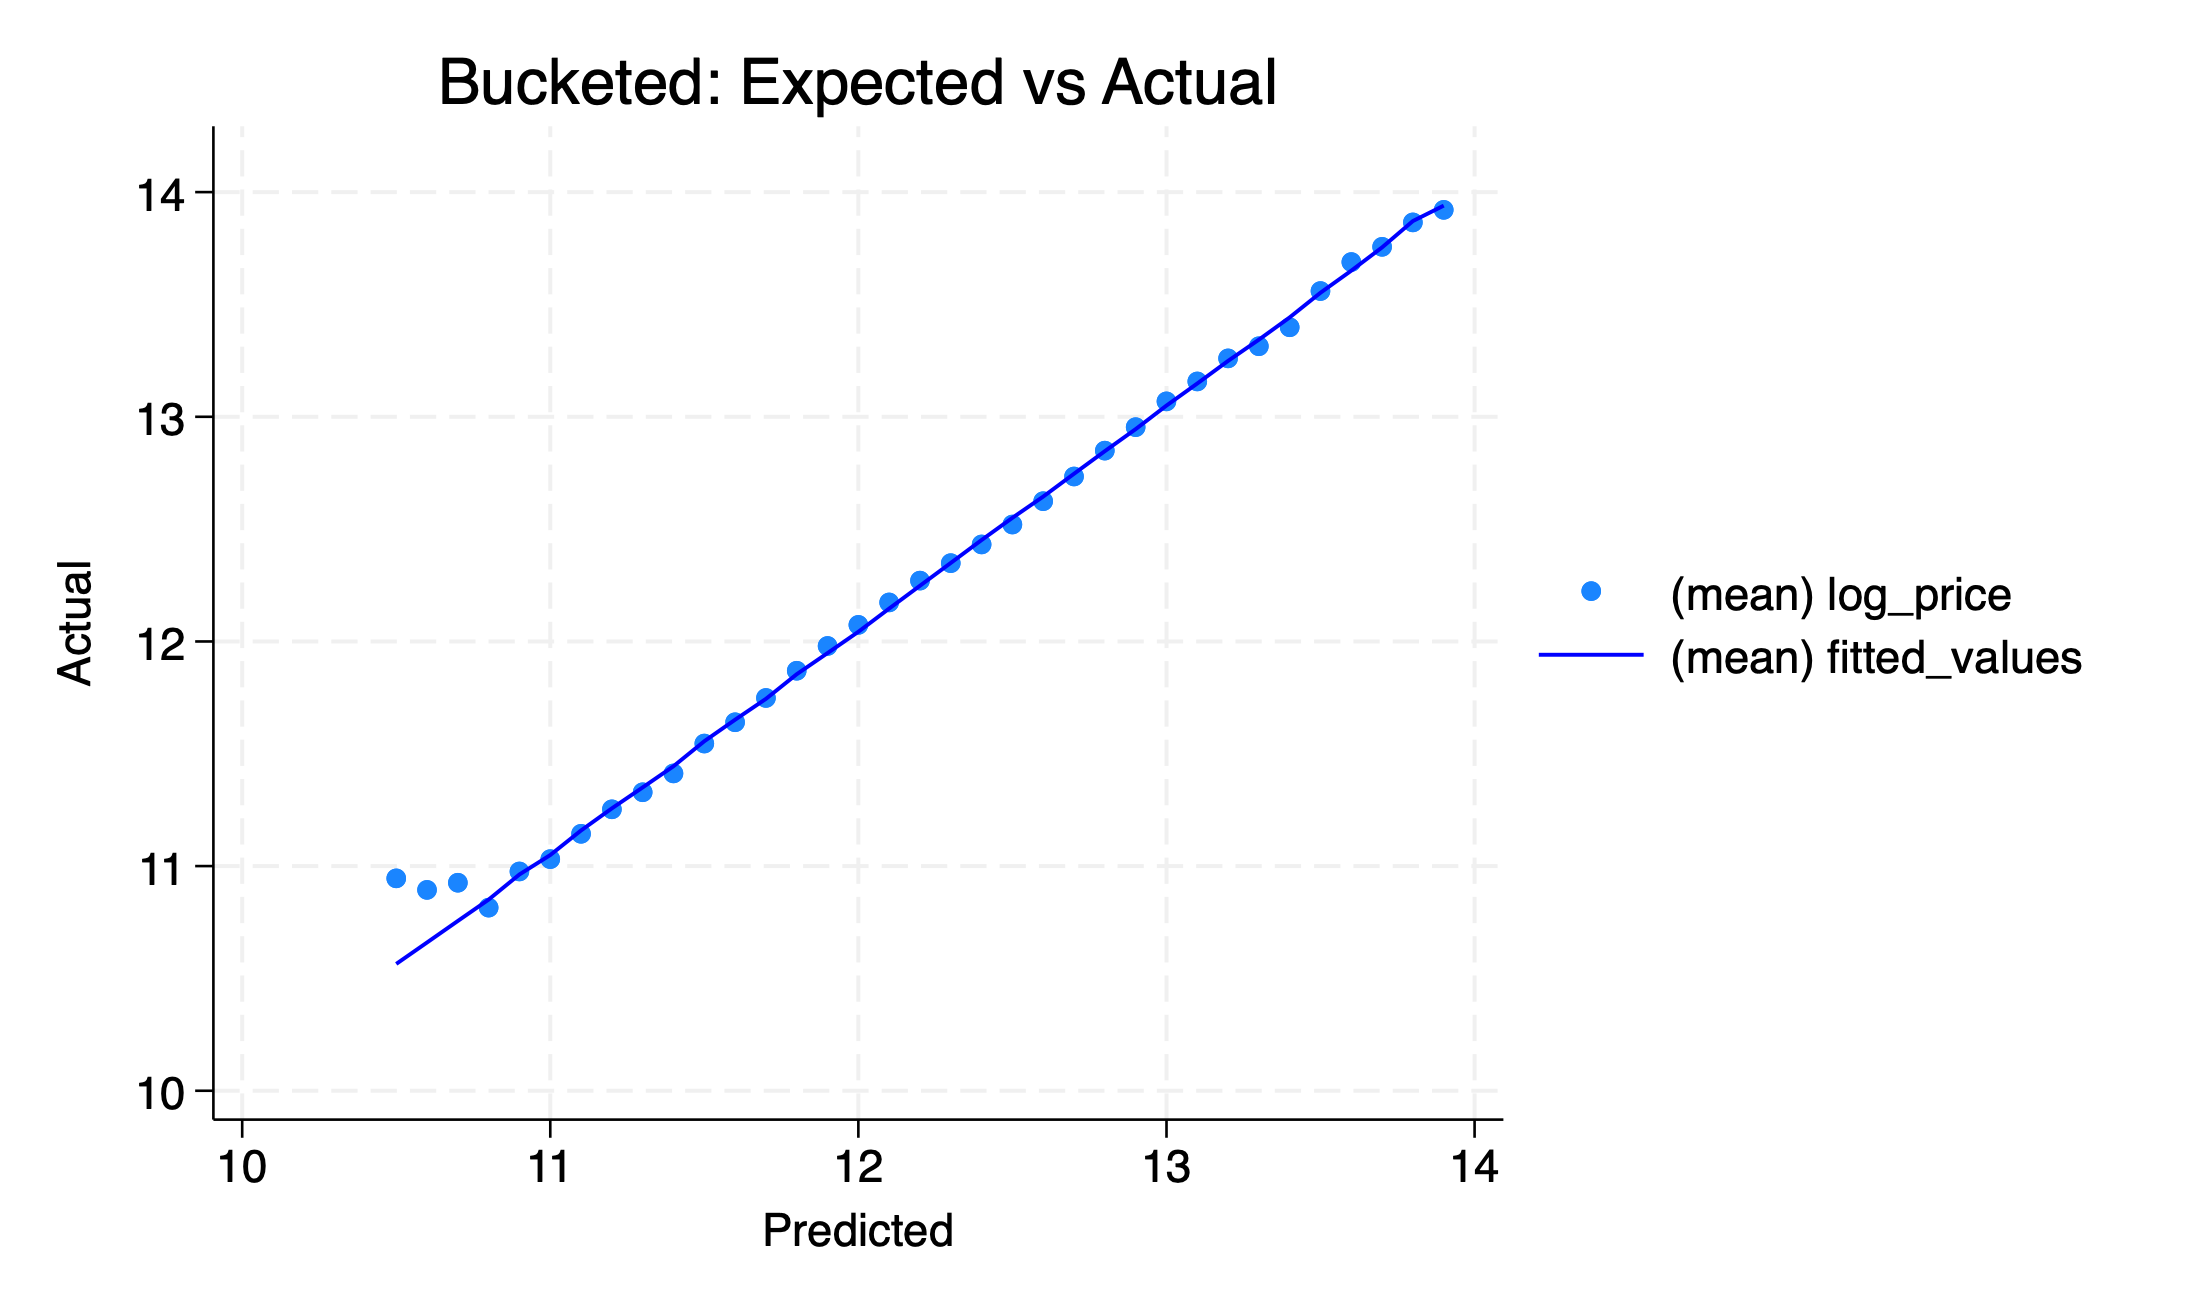
\includegraphics[width=0.8\textwidth]{../figs/bucketed_dummy_expected_vs_actual.png}
    \caption{Bucketed Expected vs Actual plot for the multivariate regression with dummy. The expected values are bucketed into 10 bins and the actual values are averaged within each bin
    we do this because with over 340000 observations the plots otherwise are difficult to interpret.
    Results are from the regression in Specification \ref{eq:dummy_multivariate_linear_regression}.}
    \label{MV_dummy_bucketed_predicted_vs_actual}
\end{figure}

% Figure showing fitted vs residuals for multivariate regression with dummy (../figs/dummy_fitted_vs_residuals.png). Label: MV_dummy_fitted_vs_residuals
\begin{figure}
    \centering
    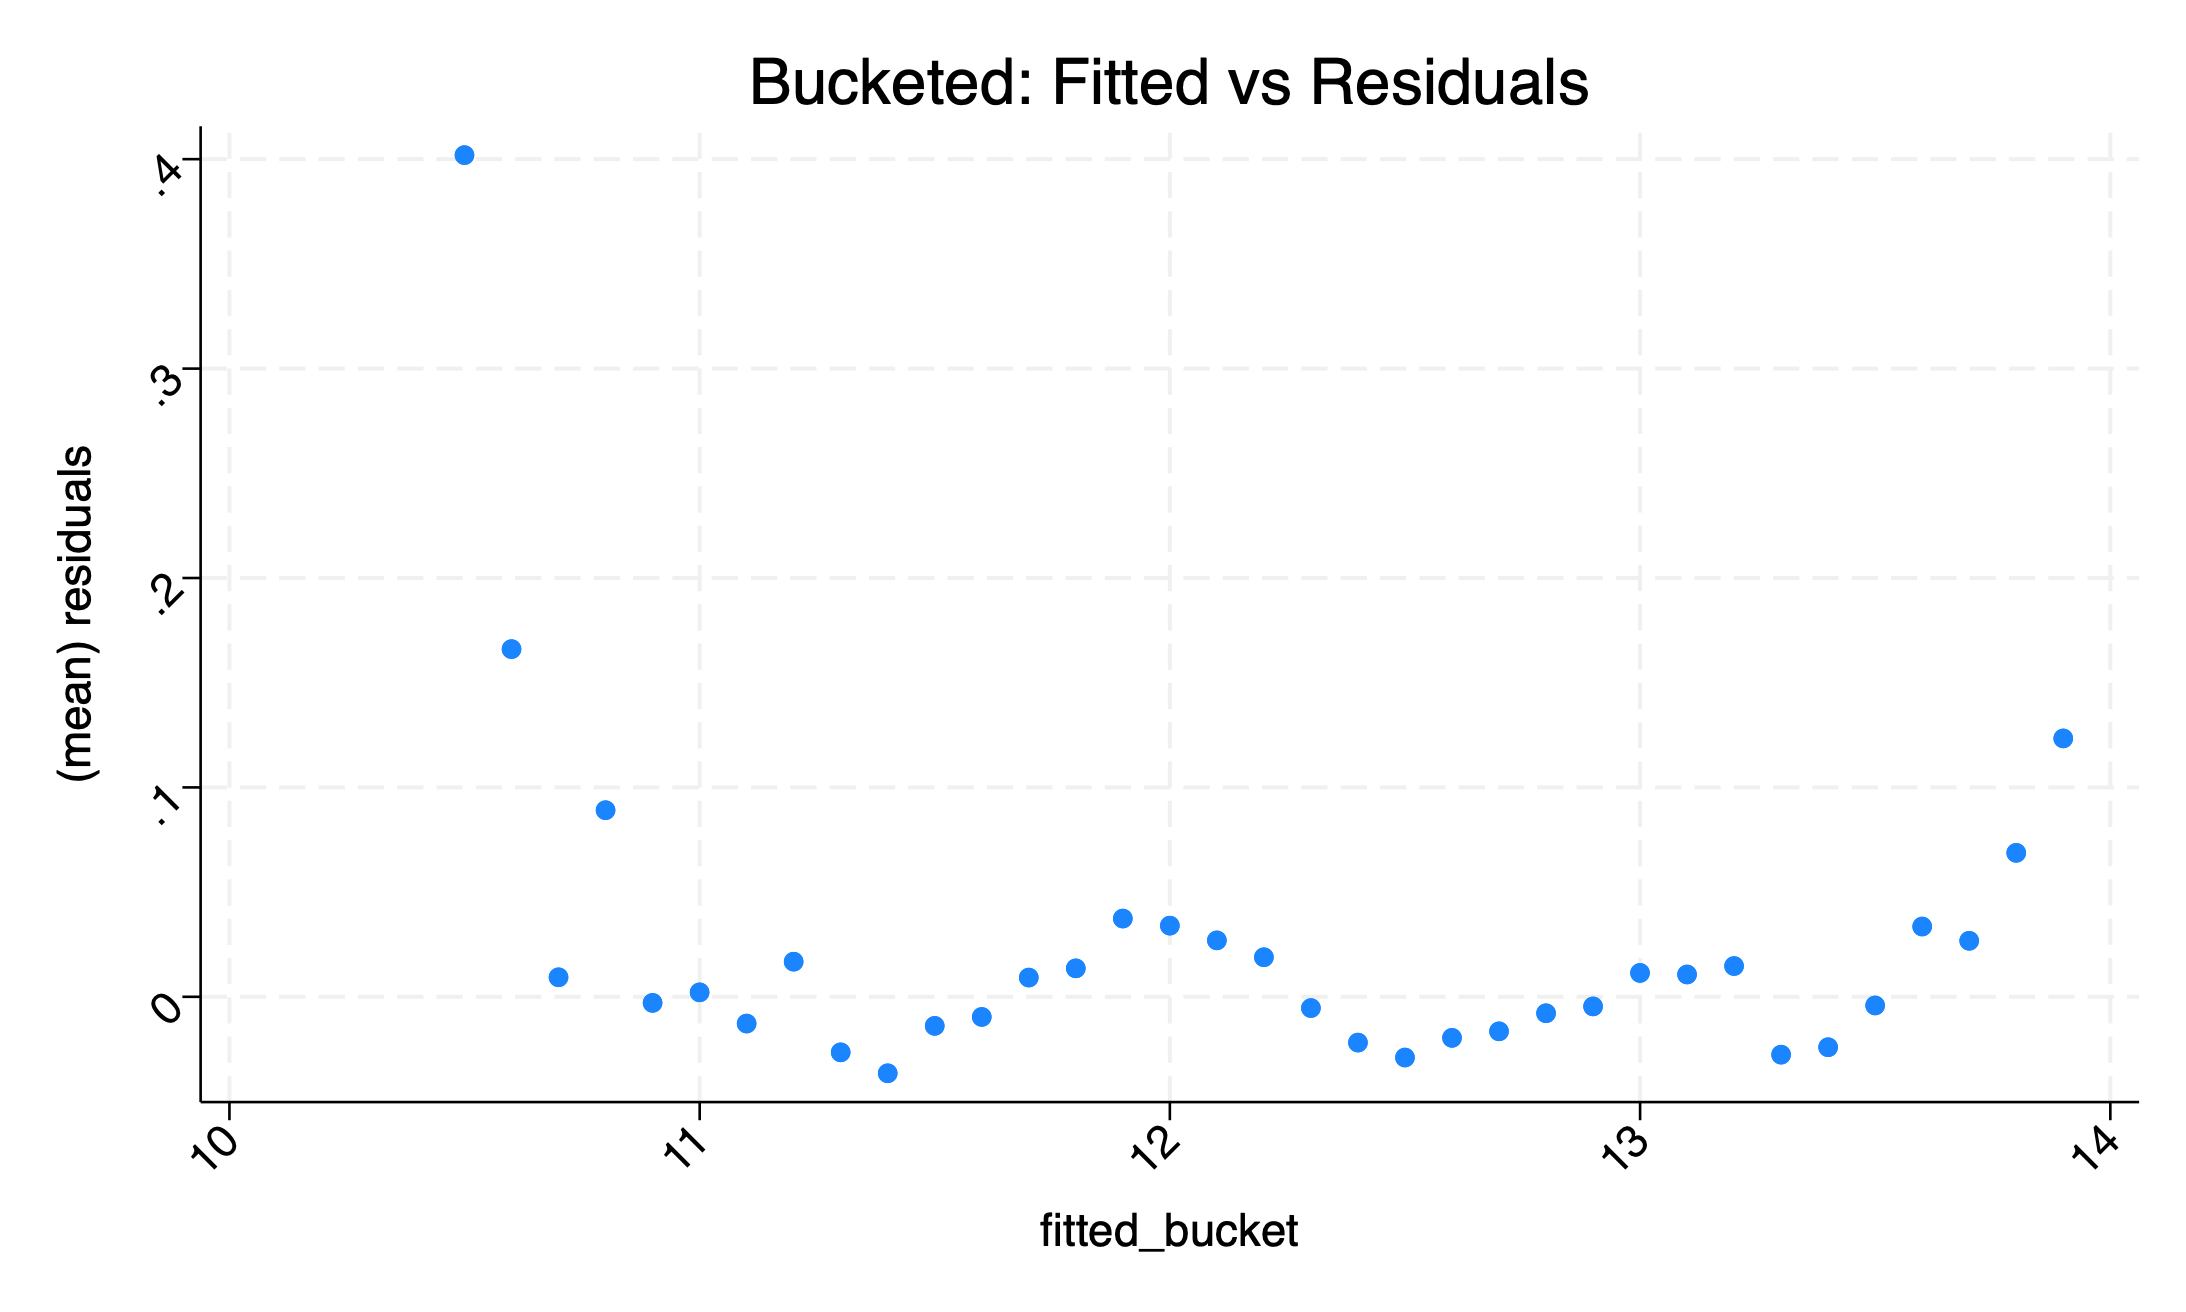
\includegraphics[width=0.8\textwidth]{../figs/dummy_fitted_vs_residuals.png}
    \caption{Fitted vs Residuals plot for the multivariate regression with dummy. The residuals are distributed randomly around 0 apart from at the lower tail where they break down.
    Results are after bucketing predicteds into bins for easier interpretation.
    Results are from the regression in Specification \ref{eq:dummy_multivariate_linear_regression}.}
    \label{MV_dummy_fitted_vs_residuals}
\end{figure}

\newpage
\subsection{Data Summary Statistics}
% Import continuous summary statistics table (../tables/numeric_MV_summary_stats.tex). Label is continuous_summary_stats
{
\def\sym#1{\ifmmode^{#1}\else\(^{#1}\)\fi}
\begin{longtable}{l*{1}{ccccc}}
\caption{Numeric Variables Summary Statistics}\\
\toprule\endfirsthead\midrule\endhead\midrule\endfoot\endlastfoot
                    &\multicolumn{5}{c}{(1)}                                         \\
                    &\multicolumn{5}{c}{}                                            \\
                    &        mean&          sd&         Var&         min&         max\\
\midrule
Min\_dist            &    2821.537&    2915.578&     8500594&    5.747817&    10141.07\\
min\_dist\_squared    &    1.65e+07&    2.83e+07&    8.00e+14&     33.0374&    1.03e+08\\
log\_price           &     12.3983&    .8569691&     .734396&     9.25913&    18.76283\\
\midrule
Observations        &      347373&            &            &            &            \\
\bottomrule
\end{longtable}
\label{tab:continuous_summary_stats}
}

\label{tab:continuous_summary_stats}

% Import Old/New summary statistics table (../tables/non_nymeric_summary_stats_ON.tex). Label is summary_ON
{
\def\sym#1{\ifmmode^{#1}\else\(^{#1}\)\fi}
\begin{longtable}{l*{1}{cc}}
\caption{Old/New Summary Statistics}\\
\toprule\endfirsthead\midrule\endhead\midrule\endfoot\endlastfoot
                    &\multicolumn{2}{c}{(1)}  \\
                    &\multicolumn{2}{c}{Old/New}\\
                    &           b&         pct\\
\midrule
N                   &      334362&    96.25446\\
Y                   &       13011&    3.745542\\
Total               &      347373&         100\\
\midrule
Observations        &      347373&            \\
\bottomrule
\end{longtable}
}

\label{tab:summary_ON}

% Import district summary statistics table (../tables/non_numeric_summary_stats_district.tex). Label is summary_district
{
\def\sym#1{\ifmmode^{#1}\else\(^{#1}\)\fi}
\begin{longtable}{l*{1}{cc}}
\caption{District Summary Statistics}\\
\toprule\endfirsthead\midrule\endhead\midrule\endfoot\endlastfoot
                    &\multicolumn{2}{c}{(1)}  \\
                    &\multicolumn{2}{c}{District}\\
                    &           b&         pct\\
\midrule
BARKING AND DAGENHAM&        6773&    1.949777\\
BARNET              &       13020&    3.748132\\
BEXLEY              &       11626&    3.346835\\
BRENT               &        8631&    2.484649\\
BROMLEY             &       17304&    4.981389\\
CAMDEN              &        8276&    2.382453\\
CITY OF LONDON      &         434&    .1249377\\
CITY OF WESTMINSTER &        9881&    2.844493\\
CROYDON             &       17283&    4.975344\\
EALING              &       11824&    3.403834\\
ENFIELD             &       13130&    3.779799\\
GREENWICH           &       10877&    3.131216\\
HACKNEY             &        7398&    2.129699\\
HAMMERSMITH AND FULHAM&        7949&    2.288318\\
HARINGEY            &        9809&    2.823766\\
HARROW              &        7131&    2.052837\\
HAVERING            &       11603&    3.340214\\
HILLINGDON          &       12621&     3.63327\\
HOUNSLOW            &        9267&    2.667738\\
ISLINGTON           &        7174&    2.065215\\
KENSINGTON AND CHELSEA&        8030&    2.311636\\
KINGSTON UPON THAMES&        8255&    2.376408\\
LAMBETH             &       14930&    4.297974\\
LEWISHAM            &       13391&    3.854934\\
MERTON              &       10079&    2.901492\\
NEWHAM              &        9985&    2.874432\\
REDBRIDGE           &       10658&    3.068172\\
RICHMOND UPON THAMES&       11298&    3.252412\\
SOUTHWARK           &       10059&    2.895735\\
SUTTON              &       10342&    2.977203\\
TOWER HAMLETS       &        6635&    1.910051\\
WALTHAM FOREST      &       12275&    3.533666\\
WANDSWORTH          &       19425&    5.591972\\
Total               &      347373&         100\\
\midrule
Observations        &      347373&            \\
\bottomrule
\end{longtable}
\label{tab:summary_district}
}

\label{tab:summary_district}

% Import year summary statistics table (../tables/non_numeric_summary_stats_year.tex). Label is summary_year
{
\def\sym#1{\ifmmode^{#1}\else\(^{#1}\)\fi}
\begin{longtable}{l*{1}{cc}}
\caption{Year Summary Statistics}\\
\toprule\endfirsthead\midrule\endhead\midrule\endfoot\endlastfoot
                    &\multicolumn{2}{c}{(1)}  \\
                    &\multicolumn{2}{c}{Year} \\
                    &           b&         pct\\
\midrule
1995                &       11273&    3.245215\\
1996                &       13798&    3.972099\\
1997                &       15791&    4.545834\\
1998                &       14966&    4.308337\\
1999                &       17317&    4.985131\\
2000                &       15518&    4.467244\\
2001                &       17110&    4.925541\\
2002                &       18197&    5.238461\\
2003                &       15726&    4.527122\\
2004                &       16029&    4.614348\\
2005                &       13882&    3.996281\\
2006                &       17206&    4.953177\\
2007                &       16474&    4.742453\\
2008                &        7402&    2.130851\\
2009                &        6962&    2.004186\\
2010                &        8703&    2.505376\\
2011                &        8340&    2.400877\\
2012                &        8537&    2.457589\\
2013                &       10055&    2.894583\\
2014                &       11275&    3.245791\\
2015                &       10621&     3.05752\\
2016                &        9442&    2.718116\\
2017                &        8588&     2.47227\\
2018                &        8278&    2.383029\\
2019                &        7836&    2.255788\\
2020                &        7420&    2.136032\\
2021                &       11412&    3.285229\\
2022                &        9337&    2.687889\\
2023                &        6825&    1.964747\\
2024                &        3053&    .8788824\\
Total               &      347373&         100\\
\midrule
Observations        &      347373&            \\
\bottomrule
\end{longtable}
\label{tab:summary_year}
}

\label{tab:summary_year}

\newpage
\subsection{Extensive Regression Results}
% Import simple regression table (../tables/simple_regression_table.tex). Label is full_simple_regression_results
{
\def\sym#1{\ifmmode^{#1}\else\(^{#1}\)\fi}
\begin{longtable}{l*{1}{c}}
\caption{Regression Results}\\
\toprule\endfirsthead\midrule\endhead\midrule\endfoot\endlastfoot
                    &\multicolumn{1}{c}{(1)}\\
                    &\multicolumn{1}{c}{log\_price}\\
\midrule
Min\_dist            &  -0.0000441\sym{***}\\
                    &(0.000000470)         \\
\addlinespace
Constant            &       12.52\sym{***}\\
                    &   (0.00208)         \\
\midrule
R-squared           &      0.0225         \\
Observations        &      347373         \\
\bottomrule
\multicolumn{2}{l}{\footnotesize Standard errors in parentheses}\\
\multicolumn{2}{l}{\footnotesize \sym{*} \(p<0.05\), \sym{**} \(p<0.01\), \sym{***} \(p<0.001\)}\\
\end{longtable}
}

\label{tab:full_simple_regression_results}

% Import simple regression table with dummy (../tables/simple_regression_table_w_dummy.tex). Label is full_simple_regression_results_w_dummy
{
\def\sym#1{\ifmmode^{#1}\else\(^{#1}\)\fi}
\begin{longtable}{l*{1}{c}}
\caption{Regression Results}\\
\toprule\endfirsthead\midrule\endhead\midrule\endfoot\endlastfoot
                    &\multicolumn{1}{c}{(1)}\\
                    &\multicolumn{1}{c}{log\_price}\\
\midrule
Min\_dist            &       0.314\sym{***}\\
                    &   (0.00283)         \\
\addlinespace
Constant            &       12.22\sym{***}\\
                    &   (0.00202)         \\
\midrule
Observations        &      347373         \\
\bottomrule
\multicolumn{2}{l}{\footnotesize Standard errors in parentheses}\\
\multicolumn{2}{l}{\footnotesize \sym{*} \(p<0.05\), \sym{**} \(p<0.01\), \sym{***} \(p<0.001\)}\\
\end{longtable}
}

\label{tab:full_simple_regression_results_w_dummy}

% Import full multivariate regression table (../tables/full_MV_regression_results.tex)
{
\def\sym#1{\ifmmode^{#1}\else\(^{#1}\)\fi}
\begin{longtable}{l*{1}{c}}
\caption{Regression Results}\\
\toprule\endfirsthead\midrule\endhead\midrule\endfoot\endlastfoot
                    &\multicolumn{1}{c}{(1)}\\
                    &\multicolumn{1}{c}{log\_price}\\
\midrule
Min\_dist            &   -0.000124\sym{***}\\
                    &(0.00000144)         \\
\addlinespace
min\_dist\_squared    &    1.07e-08\sym{***}\\
                    &  (1.35e-10)         \\
\addlinespace
N                   &           0         \\
                    &         (.)         \\
\addlinespace
Y                   &       0.116\sym{***}\\
                    &   (0.00475)         \\
\addlinespace
Year=1995           &           0         \\
                    &         (.)         \\
\addlinespace
Year=1996           &      0.0609\sym{***}\\
                    &   (0.00657)         \\
\addlinespace
Year=1997           &       0.191\sym{***}\\
                    &   (0.00645)         \\
\addlinespace
Year=1998           &       0.319\sym{***}\\
                    &   (0.00649)         \\
\addlinespace
Year=1999           &       0.483\sym{***}\\
                    &   (0.00621)         \\
\addlinespace
Year=2000           &       0.660\sym{***}\\
                    &   (0.00636)         \\
\addlinespace
Year=2001           &       0.782\sym{***}\\
                    &   (0.00612)         \\
\addlinespace
Year=2002           &       0.941\sym{***}\\
                    &   (0.00598)         \\
\addlinespace
Year=2003           &       1.062\sym{***}\\
                    &   (0.00601)         \\
\addlinespace
Year=2004           &       1.136\sym{***}\\
                    &   (0.00594)         \\
\addlinespace
Year=2005           &       1.183\sym{***}\\
                    &   (0.00612)         \\
\addlinespace
Year=2006           &       1.256\sym{***}\\
                    &   (0.00595)         \\
\addlinespace
Year=2007           &       1.382\sym{***}\\
                    &   (0.00603)         \\
\addlinespace
Year=2008           &       1.384\sym{***}\\
                    &   (0.00729)         \\
\addlinespace
Year=2009           &       1.359\sym{***}\\
                    &   (0.00770)         \\
\addlinespace
Year=2010           &       1.437\sym{***}\\
                    &   (0.00738)         \\
\addlinespace
Year=2011           &       1.456\sym{***}\\
                    &   (0.00755)         \\
\addlinespace
Year=2012           &       1.503\sym{***}\\
                    &   (0.00740)         \\
\addlinespace
Year=2013           &       1.555\sym{***}\\
                    &   (0.00722)         \\
\addlinespace
Year=2014           &       1.673\sym{***}\\
                    &   (0.00725)         \\
\addlinespace
Year=2015           &       1.772\sym{***}\\
                    &   (0.00731)         \\
\addlinespace
Year=2016           &       1.847\sym{***}\\
                    &   (0.00763)         \\
\addlinespace
Year=2017           &       1.877\sym{***}\\
                    &   (0.00839)         \\
\addlinespace
Year=2018           &       1.897\sym{***}\\
                    &   (0.00845)         \\
\addlinespace
Year=2019           &       1.902\sym{***}\\
                    &   (0.00861)         \\
\addlinespace
Year=2020           &       1.956\sym{***}\\
                    &   (0.00885)         \\
\addlinespace
Year=2021           &       1.977\sym{***}\\
                    &   (0.00739)         \\
\addlinespace
Year=2022           &       2.037\sym{***}\\
                    &   (0.00821)         \\
\addlinespace
Year=2023           &       2.013\sym{***}\\
                    &   (0.00888)         \\
\addlinespace
Year=2024           &       2.004\sym{***}\\
                    &    (0.0113)         \\
\addlinespace
BARKING AND DAGENHAM&           0         \\
                    &         (.)         \\
\addlinespace
BARNET              &       0.626\sym{***}\\
                    &   (0.00636)         \\
\addlinespace
BEXLEY              &       0.316\sym{***}\\
                    &   (0.00694)         \\
\addlinespace
BRENT               &       0.481\sym{***}\\
                    &   (0.00698)         \\
\addlinespace
BROMLEY             &       0.550\sym{***}\\
                    &   (0.00765)         \\
\addlinespace
CAMDEN              &       0.959\sym{***}\\
                    &   (0.00835)         \\
\addlinespace
CITY OF LONDON      &       0.806\sym{***}\\
                    &    (0.0370)         \\
\addlinespace
CITY OF WESTMINSTER &       1.153\sym{***}\\
                    &   (0.00916)         \\
\addlinespace
CROYDON             &       0.399\sym{***}\\
                    &   (0.00670)         \\
\addlinespace
EALING              &       0.531\sym{***}\\
                    &   (0.00615)         \\
\addlinespace
ENFIELD             &       0.450\sym{***}\\
                    &   (0.00609)         \\
\addlinespace
GREENWICH           &       0.464\sym{***}\\
                    &   (0.00654)         \\
\addlinespace
HACKNEY             &       0.618\sym{***}\\
                    &   (0.00711)         \\
\addlinespace
HAMMERSMITH AND FULHAM&       0.926\sym{***}\\
                    &   (0.00778)         \\
\addlinespace
HARINGEY            &       0.508\sym{***}\\
                    &   (0.00694)         \\
\addlinespace
HARROW              &       0.464\sym{***}\\
                    &   (0.00696)         \\
\addlinespace
HAVERING            &       0.353\sym{***}\\
                    &   (0.00549)         \\
\addlinespace
HILLINGDON          &       0.386\sym{***}\\
                    &   (0.00547)         \\
\addlinespace
HOUNSLOW            &       0.474\sym{***}\\
                    &   (0.00675)         \\
\addlinespace
ISLINGTON           &       0.783\sym{***}\\
                    &   (0.00783)         \\
\addlinespace
KENSINGTON AND CHELSEA&       1.430\sym{***}\\
                    &    (0.0102)         \\
\addlinespace
KINGSTON UPON THAMES&       0.790\sym{***}\\
                    &   (0.00748)         \\
\addlinespace
LAMBETH             &       0.613\sym{***}\\
                    &   (0.00584)         \\
\addlinespace
LEWISHAM            &       0.508\sym{***}\\
                    &   (0.00636)         \\
\addlinespace
MERTON              &       0.612\sym{***}\\
                    &   (0.00705)         \\
\addlinespace
NEWHAM              &       0.129\sym{***}\\
                    &   (0.00544)         \\
\addlinespace
REDBRIDGE           &       0.340\sym{***}\\
                    &   (0.00577)         \\
\addlinespace
RICHMOND UPON THAMES&       1.002\sym{***}\\
                    &   (0.00689)         \\
\addlinespace
SOUTHWARK           &       0.620\sym{***}\\
                    &   (0.00678)         \\
\addlinespace
SUTTON              &       0.521\sym{***}\\
                    &   (0.00618)         \\
\addlinespace
TOWER HAMLETS       &       0.530\sym{***}\\
                    &   (0.00714)         \\
\addlinespace
WALTHAM FOREST      &       0.272\sym{***}\\
                    &   (0.00539)         \\
\addlinespace
WANDSWORTH          &       0.804\sym{***}\\
                    &   (0.00570)         \\
\addlinespace
Constant            &       10.83\sym{***}\\
                    &   (0.00641)         \\
\midrule
Observations        &      347373         \\
\bottomrule
\multicolumn{2}{l}{\footnotesize Standard errors in parentheses}\\
\multicolumn{2}{l}{\footnotesize \sym{*} \(p<0.05\), \sym{**} \(p<0.01\), \sym{***} \(p<0.001\)}\\
\end{longtable}
}

\label{tab:full_MV_regression_results}

% Import full multivariate regression table with dummy (../tables/full_MV_regression_results_w_dummy.tex)
{
\def\sym#1{\ifmmode^{#1}\else\(^{#1}\)\fi}
\begin{longtable}{l*{1}{c}}
\caption{Regression results using the close/far dummyMin\_dist is either 0 or 1. Shows us that the dummy effect is still economically and statistically significant in-context with our controls.}\\
\toprule\endfirsthead\midrule\endhead\midrule\endfoot\endlastfoot
                    &\multicolumn{1}{c}{(1)}\\
                    &\multicolumn{1}{c}{log\_price}\\
\midrule
Min\_dist=0          &           0         \\
                    &         (.)         \\
\addlinespace
Min\_dist=1          &       0.189\sym{***}\\
                    &   (0.00290)         \\
\addlinespace
N                   &           0         \\
                    &         (.)         \\
\addlinespace
Y                   &       0.119\sym{***}\\
                    &   (0.00476)         \\
\addlinespace
Year=1995           &           0         \\
                    &         (.)         \\
\addlinespace
Year=1996           &      0.0605\sym{***}\\
                    &   (0.00663)         \\
\addlinespace
Year=1997           &       0.192\sym{***}\\
                    &   (0.00649)         \\
\addlinespace
Year=1998           &       0.321\sym{***}\\
                    &   (0.00663)         \\
\addlinespace
Year=1999           &       0.482\sym{***}\\
                    &   (0.00655)         \\
\addlinespace
Year=2000           &       0.661\sym{***}\\
                    &   (0.00681)         \\
\addlinespace
Year=2001           &       0.782\sym{***}\\
                    &   (0.00684)         \\
\addlinespace
Year=2002           &       0.939\sym{***}\\
                    &   (0.00696)         \\
\addlinespace
Year=2003           &       1.060\sym{***}\\
                    &   (0.00732)         \\
\addlinespace
Year=2004           &       1.135\sym{***}\\
                    &   (0.00752)         \\
\addlinespace
Year=2005           &       1.182\sym{***}\\
                    &   (0.00793)         \\
\addlinespace
Year=2006           &       1.255\sym{***}\\
                    &   (0.00795)         \\
\addlinespace
Year=2007           &       1.380\sym{***}\\
                    &   (0.00827)         \\
\addlinespace
Year=2008           &       1.384\sym{***}\\
                    &   (0.00966)         \\
\addlinespace
Year=2009           &       1.360\sym{***}\\
                    &    (0.0100)         \\
\addlinespace
Year=2010           &       1.438\sym{***}\\
                    &   (0.00992)         \\
\addlinespace
Year=2011           &       1.457\sym{***}\\
                    &    (0.0103)         \\
\addlinespace
Year=2012           &       1.502\sym{***}\\
                    &    (0.0105)         \\
\addlinespace
Year=2013           &       1.554\sym{***}\\
                    &    (0.0106)         \\
\addlinespace
Year=2014           &       1.673\sym{***}\\
                    &    (0.0109)         \\
\addlinespace
Year=2015           &       1.771\sym{***}\\
                    &    (0.0113)         \\
\addlinespace
Year=2016           &       1.846\sym{***}\\
                    &    (0.0117)         \\
\addlinespace
Year=2017           &       1.877\sym{***}\\
                    &    (0.0122)         \\
\addlinespace
Year=2018           &       1.899\sym{***}\\
                    &    (0.0126)         \\
\addlinespace
Year=2019           &       1.903\sym{***}\\
                    &    (0.0130)         \\
\addlinespace
Year=2020           &       1.957\sym{***}\\
                    &    (0.0134)         \\
\addlinespace
Year=2021           &       1.979\sym{***}\\
                    &    (0.0133)         \\
\addlinespace
Year=2022           &       2.035\sym{***}\\
                    &    (0.0139)         \\
\addlinespace
Year=2023           &       2.010\sym{***}\\
                    &    (0.0146)         \\
\addlinespace
Year=2024           &       2.005\sym{***}\\
                    &    (0.0166)         \\
\addlinespace
BARKING AND DAGENHAM&           0         \\
                    &         (.)         \\
\addlinespace
BARNET              &       2.225         \\
                    &     (1.945)         \\
\addlinespace
BEXLEY              &       5.123\sym{**} \\
                    &     (1.974)         \\
\addlinespace
BRENT               &      -19.32\sym{***}\\
                    &     (2.103)         \\
\addlinespace
BROMLEY             &       5.577\sym{**} \\
                    &     (1.858)         \\
\addlinespace
CAMDEN              &      -6.402\sym{**} \\
                    &     (2.130)         \\
\addlinespace
CITY OF LONDON      &      -23.19\sym{**} \\
                    &     (7.644)         \\
\addlinespace
CITY OF WESTMINSTER &      -17.68\sym{***}\\
                    &     (2.043)         \\
\addlinespace
CROYDON             &       4.450\sym{*}  \\
                    &     (1.851)         \\
\addlinespace
EALING              &      -2.391         \\
                    &     (1.985)         \\
\addlinespace
ENFIELD             &       2.017         \\
                    &     (1.944)         \\
\addlinespace
GREENWICH           &      -4.107\sym{*}  \\
                    &     (2.007)         \\
\addlinespace
HACKNEY             &      -29.34\sym{***}\\
                    &     (2.163)         \\
\addlinespace
HAMMERSMITH AND FULHAM&      -4.642\sym{*}  \\
                    &     (2.135)         \\
\addlinespace
HARINGEY            &      -12.52\sym{***}\\
                    &     (2.030)         \\
\addlinespace
HARROW              &       5.490\sym{*}  \\
                    &     (2.198)         \\
\addlinespace
HAVERING            &       10.56\sym{***}\\
                    &     (1.962)         \\
\addlinespace
HILLINGDON          &       6.397\sym{**} \\
                    &     (1.954)         \\
\addlinespace
HOUNSLOW            &       5.913\sym{**} \\
                    &     (2.080)         \\
\addlinespace
ISLINGTON           &      -5.364\sym{*}  \\
                    &     (2.195)         \\
\addlinespace
KENSINGTON AND CHELSEA&      -12.54\sym{***}\\
                    &     (2.152)         \\
\addlinespace
KINGSTON UPON THAMES&       3.984         \\
                    &     (2.123)         \\
\addlinespace
LAMBETH             &      -9.866\sym{***}\\
                    &     (1.897)         \\
\addlinespace
LEWISHAM            &      -17.46\sym{***}\\
                    &     (1.927)         \\
\addlinespace
MERTON              &      -1.193         \\
                    &     (2.029)         \\
\addlinespace
NEWHAM              &      -14.91\sym{***}\\
                    &     (2.059)         \\
\addlinespace
REDBRIDGE           &      -0.242         \\
                    &     (2.023)         \\
\addlinespace
RICHMOND UPON THAMES&       8.947\sym{***}\\
                    &     (1.985)         \\
\addlinespace
SOUTHWARK           &      -18.27\sym{***}\\
                    &     (2.031)         \\
\addlinespace
SUTTON              &       8.082\sym{***}\\
                    &     (2.017)         \\
\addlinespace
TOWER HAMLETS       &       1.581         \\
                    &     (2.261)         \\
\addlinespace
WALTHAM FOREST      &      -23.41\sym{***}\\
                    &     (1.948)         \\
\addlinespace
WANDSWORTH          &      -3.230         \\
                    &     (1.829)         \\
\addlinespace
BARKING AND DAGENHAM $\times$ Year&    -0.00201\sym{*}  \\
                    &  (0.000911)         \\
\addlinespace
BARNET $\times$ Year&    -0.00281\sym{***}\\
                    &  (0.000719)         \\
\addlinespace
BEXLEY $\times$ Year&    -0.00439\sym{***}\\
                    &  (0.000738)         \\
\addlinespace
BRENT $\times$ Year &     0.00788\sym{***}\\
                    &  (0.000822)         \\
\addlinespace
BROMLEY $\times$ Year&    -0.00447\sym{***}\\
                    &  (0.000659)         \\
\addlinespace
CAMDEN $\times$ Year&     0.00168\sym{*}  \\
                    &  (0.000839)         \\
\addlinespace
CITY OF LONDON $\times$ Year&     0.00998\sym{**} \\
                    &   (0.00375)         \\
\addlinespace
CITY OF WESTMINSTER $\times$ Year&     0.00740\sym{***}\\
                    &  (0.000783)         \\
\addlinespace
CROYDON $\times$ Year&    -0.00402\sym{***}\\
                    &  (0.000654)         \\
\addlinespace
EALING $\times$ Year&   -0.000548         \\
                    &  (0.000746)         \\
\addlinespace
ENFIELD $\times$ Year&    -0.00280\sym{***}\\
                    &  (0.000718)         \\
\addlinespace
GREENWICH $\times$ Year&    0.000254         \\
                    &  (0.000760)         \\
\addlinespace
HACKNEY $\times$ Year&      0.0129\sym{***}\\
                    &  (0.000860)         \\
\addlinespace
HAMMERSMITH AND FULHAM $\times$ Year&    0.000783         \\
                    &  (0.000842)         \\
\addlinespace
HARINGEY $\times$ Year&     0.00448\sym{***}\\
                    &  (0.000775)         \\
\addlinespace
HARROW $\times$ Year&    -0.00451\sym{***}\\
                    &  (0.000882)         \\
\addlinespace
HAVERING $\times$ Year&    -0.00709\sym{***}\\
                    &  (0.000731)         \\
\addlinespace
HILLINGDON $\times$ Year&    -0.00500\sym{***}\\
                    &  (0.000726)         \\
\addlinespace
HOUNSLOW $\times$ Year&    -0.00472\sym{***}\\
                    &  (0.000808)         \\
\addlinespace
ISLINGTON $\times$ Year&     0.00107         \\
                    &  (0.000880)         \\
\addlinespace
KENSINGTON AND CHELSEA $\times$ Year&     0.00498\sym{***}\\
                    &  (0.000853)         \\
\addlinespace
KINGSTON UPON THAMES $\times$ Year&    -0.00362\sym{***}\\
                    &  (0.000834)         \\
\addlinespace
LAMBETH $\times$ Year&     0.00322\sym{***}\\
                    &  (0.000686)         \\
\addlinespace
LEWISHAM $\times$ Year&     0.00692\sym{***}\\
                    &  (0.000707)         \\
\addlinespace
MERTON $\times$ Year&    -0.00110         \\
                    &  (0.000774)         \\
\addlinespace
NEWHAM $\times$ Year&     0.00549\sym{***}\\
                    &  (0.000795)         \\
\addlinespace
REDBRIDGE $\times$ Year&    -0.00172\sym{*}  \\
                    &  (0.000771)         \\
\addlinespace
RICHMOND UPON THAMES $\times$ Year&    -0.00597\sym{***}\\
                    &  (0.000745)         \\
\addlinespace
SOUTHWARK $\times$ Year&     0.00740\sym{***}\\
                    &  (0.000776)         \\
\addlinespace
SUTTON $\times$ Year&    -0.00579\sym{***}\\
                    &  (0.000767)         \\
\addlinespace
TOWER HAMLETS $\times$ Year&    -0.00252\sym{**} \\
                    &  (0.000921)         \\
\addlinespace
WALTHAM FOREST $\times$ Year&     0.00979\sym{***}\\
                    &  (0.000721)         \\
\addlinespace
WANDSWORTH $\times$ Year&           0         \\
                    &         (.)         \\
\addlinespace
Constant            &       14.57\sym{***}\\
                    &     (1.826)         \\
\midrule
R-squared           &       0.631         \\
Observations        &      347373         \\
\bottomrule
\multicolumn{2}{l}{\footnotesize Standard errors in parentheses}\\
\multicolumn{2}{l}{\footnotesize \sym{*} \(p<0.05\), \sym{**} \(p<0.01\), \sym{***} \(p<0.001\)}\\
\end{longtable}
}

\label{tab:full_MV_regression_results_w_dummy}